% Chapter Template

\chapter{Monitoring Tool - Architecture} % Main chapter title

\label{Chapter3} % Change X to a consecutive number; for referencing this chapter elsewhere, use \ref{ChapterX}

\lhead{Chapter 3. \emph{Monitoring Tool - Part 1}}
\section{Requirements}
The first step of conception was to define the goals of the system. This means enumerate what the people supposed to use it want. To structure our reflection, we use a pseudo version of the \emph{Goal Model} taught by the Professor van Lamsweerde\cite{van2009requirements}. We tried to stay as close as possible from the original syntax but we may have taken some freedom to keep things simple.
\subsection{System Goals}
The main goal as suggested by the title of our thesis is to monitor and analyse the wifi network. We want to be able to knwow what happens in the network and understanding the data generate by the components. To \emph{achieve} that we will be required to understand what the controller tells in its logs files and what are the data it makes available in its \emph{Management Information Base}. Monitoring is also an active task. We shall need to analyse the quality of service experienced by an user when he uses the wifi. Beside the gathering part, we have to analyse those results and moreover being able to detect issues as soon as possible.
\begin{figure}[H]
\centering
	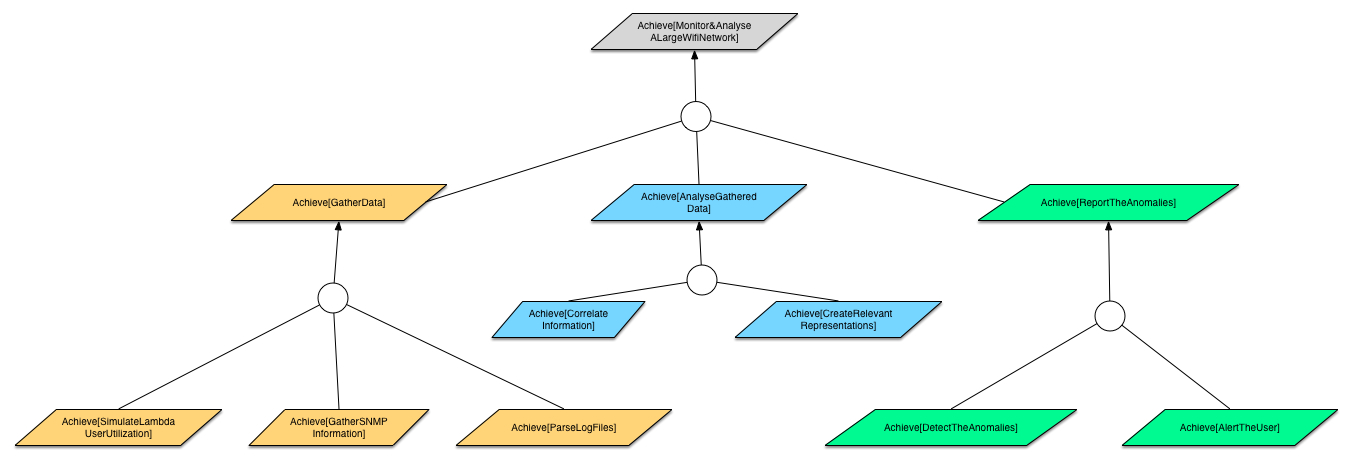
\includegraphics[width=1.1\linewidth]{Pictures/chapter3/goals.jpg}
	\caption{Pseudo Goal Model}
\end{figure}
These requirements comes from the meetings we had with the SGSI. We discuss what such a tool could use as source of information and what new data could be generate from them. It's quite important to determine what we do and how we will achieve it as soon as possible. This quite simple model will allow us to focus on one task at a time without loosing the final purpose.

\subsection{Goals Definition}
\begin{description}
  \item[Name] MonitorAndAnalyseALargeWifiNetwork
  \item[Description] The root goal of our system is to allow the administrators to understand what is currently happening on his network. The ideal would be a real-time view of the infrastructure.
\end{description}

\begin{description}
  \item[Name] GatherData
  \item[Description] To achieve a efficient monitoring we have to gatherer and centralize the available information. 
\end{description}

\begin{description}
  \item[Name] SimulateLambdaUserUtilization
  \item[Description] We need to evaluate how the users experienced the utilization of the network.
\end{description}

\begin{description}
  \item[Name] GatherSNMPInformation
  \item[Description] Record the states of the controller and the access points through time.
\end{description}

\begin{description}
  \item[Name] ParseLogFiles
  \item[Description] We have to be able to understand the information generated by the Controller, Radius and DHCP server.
\end{description}

\begin{description}
  \item[Name] AnalyseGatheredData
  \item[Description] Once the data are available, we need to analyse and make comparison between them.
\end{description}

\begin{description}
  \item[Name] CorrelateInformation
  \item[Description] We want to put related data together and generate new information.
\end{description}

\begin{description}
  \item[Name] CreateRelevantRepresentations
  \item[Description] Our results have to be understood be the users.
\end{description}

\begin{description}
  \item[Name] ReportTheAnomalies
  \item[Description] More than analyse, the system have to be able to alert the administrators of anomalies.
\end{description}

\begin{description}
  \item[Name] DetectTheAnomalies
  \item[Description] We have to define what are anomalies and use those rules to record deviant behaviour.
\end{description}

\begin{description}
  \item[Name] AlertTheUser
  \item[Description] Communicate to the users the anomalies.
\end{description}

\section{Architecture}
In our architecture system, we have two very distinct entities. The first entity, called the \textit{Gatherer}, is the one responsible for gathering information. This component handles the responsibility to keep the operational database up to date and in a consistent state. The other side of the application, the \textit{Analyser}, is managing the analysis made with all the information we have gathered. Upon these two processes, we'll add an alert system that which produce warnings when an anomalies is spotted. These three parts have to be as independent as possible but able to communicate between them efficiently. We have designed them by keeping two rules in mind: modularity and simplicity.

\subsection{Gatherer}
This part of the application is constituted of several modules that allow it to communicate with the various sources of information. Each module is responsible of a particular kind of information and each of them have to transform that piece of information in a coherent entry in the database. As the information come from heterogeneous origins, each information have to be understood and transformed into an entity that can be related to others. Without such transformation, the possible analysis would be really limited and not really interesting. We focus here on the \texttt{Achieve[GatherData]} goal and its refinement.

\subsubsection{Logs}
The first kind of information we managed to analyse was the logs files. There is one different log type per infrastructure component:
\begin{itemize}
\item Radius
\item DHCP
\item Wism (Controller)
\end{itemize}
These elements generate several logs each seconds and the main difficulty was to make a first sorting among all those data. A part of them are just informational and don't bring useful information about the state of the network. Such messages will never be used during the analysis and then they don't need to be store in the database. Another part of the logs are repetition of others. In fact, as each element produces its logs independently, some logs can overlap and represent the same information. Redundant information are useless and the same information don't need to be in the database twice. This can seems to be a unimportant issue but in consideration of the quantity of information proceed by the application, an overloading of the database can cause severe performance issue during the analysis phase.
The ideal way of gathering such information would be to load them directly from the sources at our convenience. In this way, we could manage and optimise the processing of the data.

\subsubsection{SNMP}
The SNMP protocol allows us to retrieve information on the controller in real-time. The module handling the SNMP request can update the information about the situation of each access point or any client. This bring a lot of interesting data regarding the users of the network but the main drawback is that the requests are heavy. We can't make them at any time because it requires resources from the controller and from our server. In consequence, we have to find the right balance between keeping the database update and not overloading the controller with SNMP request.
The most important information extracted are the status of every access points (AP). We can see what access point are actually associated with the controller. A lot of statistics (e.g the load of the AP) are available.
The same holds for the client associated to an access point. Each mobile station is indexed by the controller and statistics about it are hold by it.

\subsubsection{Active Monitoring}
Also, we have implemented an active monitoring tool in the form of a \texttt{C} program running on \texttt{OpenWrt} routers. The purpose of this element is to simulate a user. We can't be aware of the experience of the user by looking at SNMP request or log files. Here, we will use an unmodified version of \emph{wpa$\_$supplicant}. We simply generate connections and monitor what happens. We mostly record the time of each steps and observe which access point is chosen and what are the environment of the router. For example, we will scan the nearest access point, record their signal strength and trying to estimate the quality experienced by an user that would be in the same situation.

\subsubsection{Database}
The database have to be able of representing each kind of information and manage the links between them. It isn't hard to create entries for a log but the difficulties appear when we make link with other entities and have to keep them in a coherent state. Several questions raised when we try to designed our database. For example, if a client is no more associated with an access point, do we have to remove it from the database? Such questions can seem futile but may have deep implications on the database performance. Our choice was to clearly separate the difference domain of data. Trying to make a links between each element could create inconsistencies and making the analyse harder. That's why each category of information owns its tables and links are only made when they are present in the original data. This doesn't means that we don't cross the information, it means that we let the data independent and only compare them when we need to perform analyse. As there are plenty of way to organize them, we preferred to keep them neat and avoid to mix them in the gathering part.

\subsection{Analyser}
As the gatherer only put available information together, it doesn't bring anything new. In the other side, the analyse component will use the data and the links between them to extract useful information about the network. For example, the SNMP shows the people associated with an access point but only an analysis through time will allow us to detect and even forecast overload in the network. This component will manage the analyse on the database and storing the result over the time.

\section{Link with the Infrastructure}
As a monitoring, we need to be plug on the infrastructure. For each of data source, we have to define a point of communication in our system. The data are not centralized and we have to manage how we access them and trying to define a balance between performance and respect of the external components which host the information. For example, we can't submerge the SNMP agents with requests.

\begin{figure}[H]
\centering
	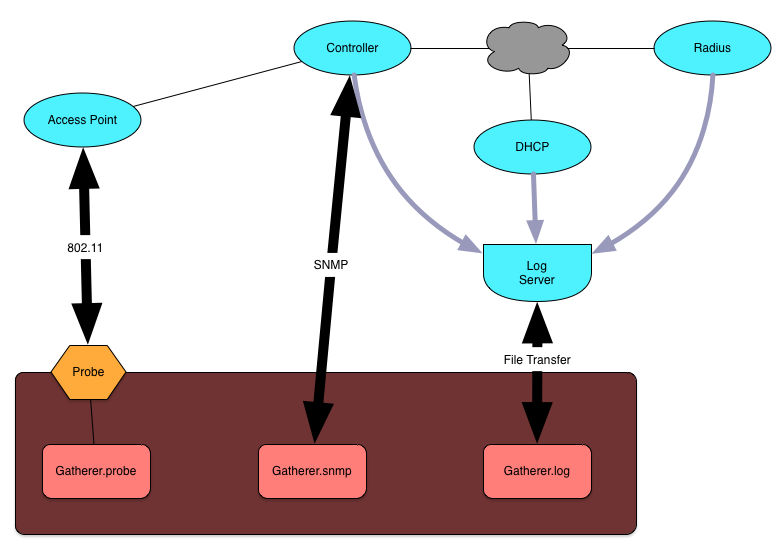
\includegraphics[width=1\linewidth]{Pictures/chapter3/interactions.jpg}
	\caption{Interconnections with the infrastructure}
\end{figure}

\subsection{Controller}
The controller hosts all the SNMP data about itself or the access points. The system will retrieve them directly on it periodically. As shown, it's the \texttt{gatherer.snmpa} that handles the transactions. As said before, there are two controllers hidden behind one virtual IP. That configuration allows to always perform the request to the same address and the active controller will answer.
\subsection{Access Points}
The probe will associate with an access point and the result will be sent to the server. There is no special configuration required as the device need to operate as a lambda user and in consequence it will simply use its driver to test the AP. 
\subsection{Log Server} 
The log files are stored on a dedicated server and the administrator retrieve them from there. In an ideal situation, we should automatise the gathering of those files and process them periodically too.
